\documentclass[aspectratio=169]{beamer}

\usetheme{Madrid}
\usepackage{booktabs}
\usepackage{graphicx}
\usepackage{array}

\title{GemmaScope SAE Layer Localization}
\subtitle{Where the model-merging refusal repair lives}
\author{Local model merging project}
\date{2026-05-22}

\begin{document}

\begin{frame}
  \titlepage
\end{frame}

\begin{frame}{Question}
  \textbf{Previous result:} selected GemmaScope MLP-SAE features over layers 12--20 can repair refusal better than random active features.

  \vspace{0.35cm}
  \textbf{New question:} is that repair concentrated in one small layer band, or distributed across multiple bands?

  \vspace{0.35cm}
  \begin{itemize}
    \item Donor/base: \texttt{google/gemma-2-2b-it}
    \item Recipient: \texttt{IlyaGusev/gemma-2-2b-it-abliterated}
    \item Site: normalized post-feedforward MLP outputs
    \item Feature selector: harmful donor-recipient SAE activation delta
  \end{itemize}
\end{frame}

\begin{frame}{Single 3-Layer Bands}
  \begin{center}
    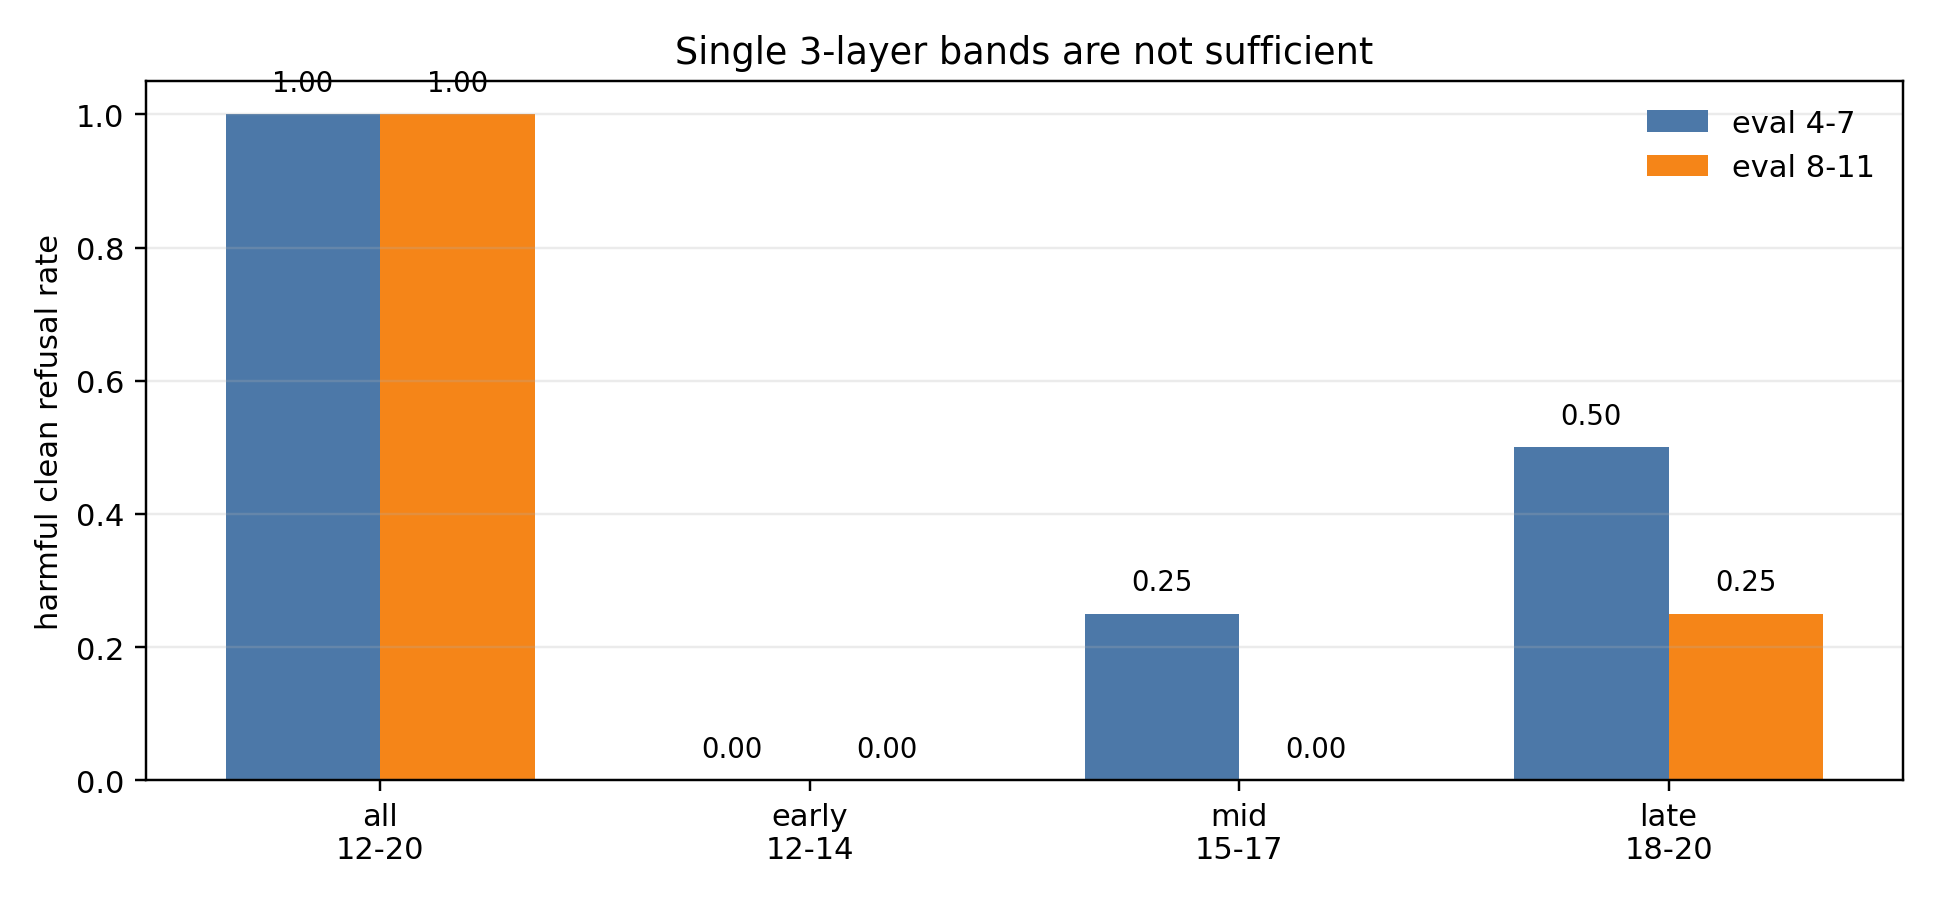
\includegraphics[width=0.86\linewidth]{figures/single_band_full_decode.png}
  \end{center}
  \vspace{-0.15cm}
  {\small Bars show harmful clean-refusal rate for full decoded SAE patches. No single 3-layer band is sufficient.}
\end{frame}

\begin{frame}{Paired Bands}
  \begin{center}
    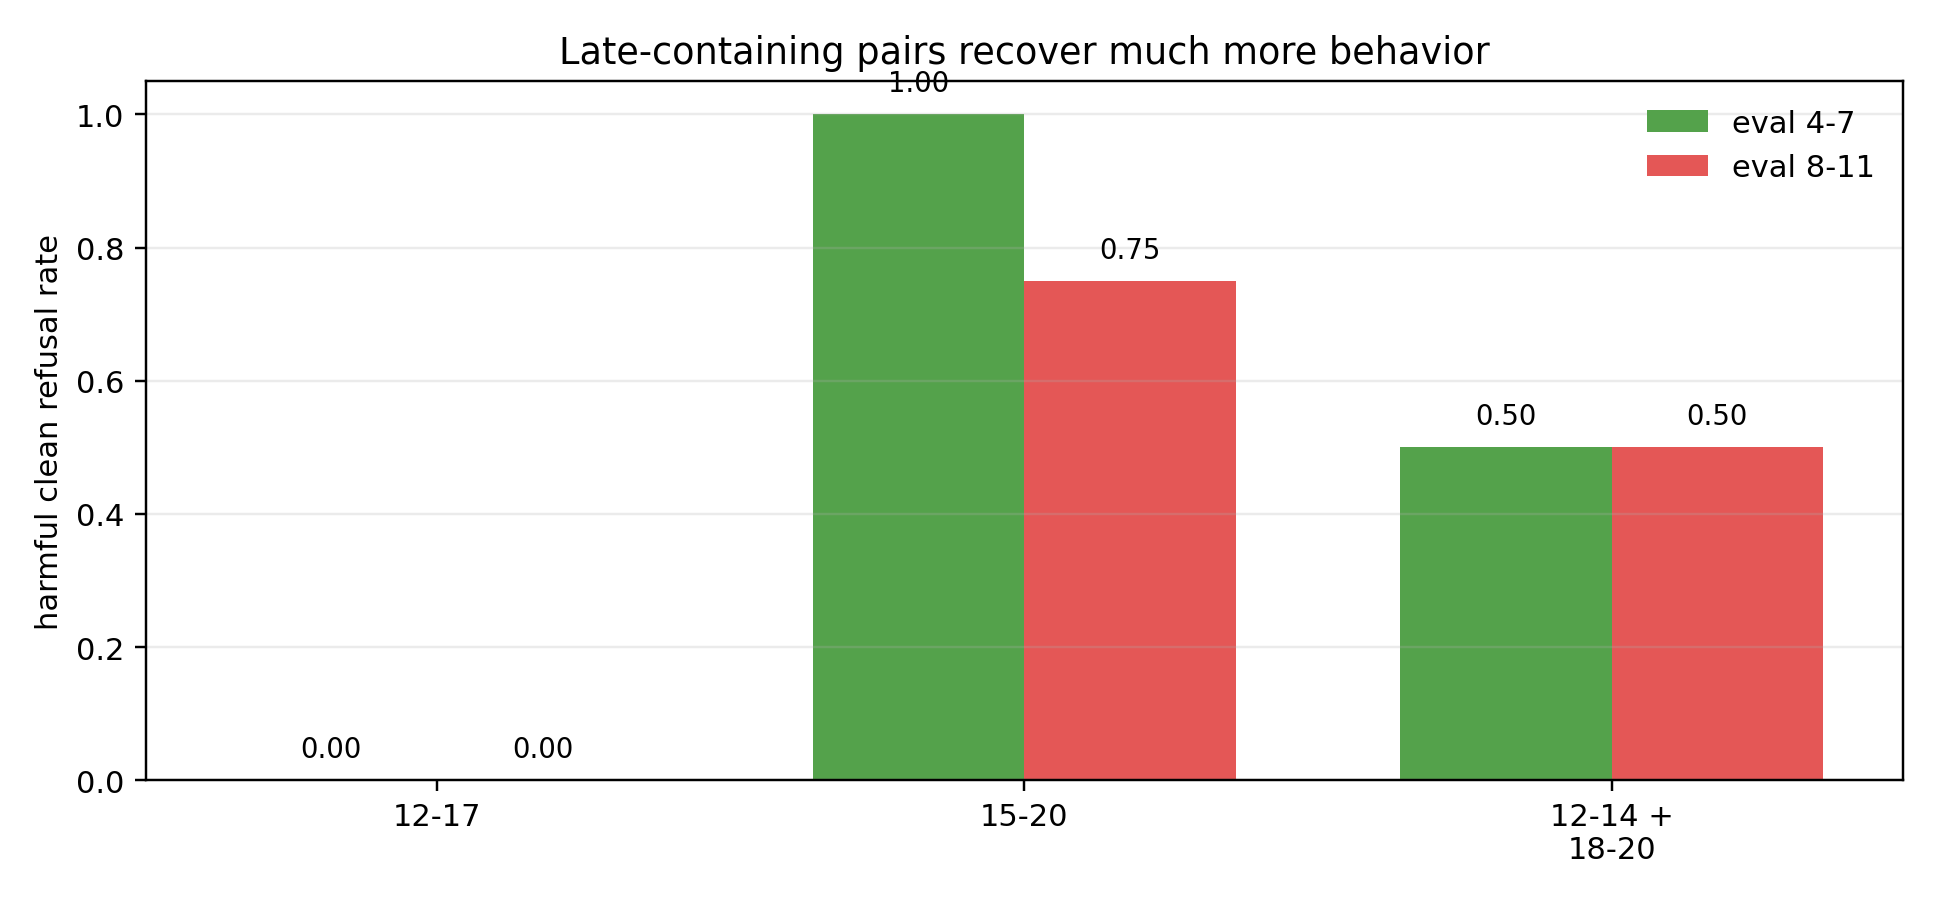
\includegraphics[width=0.86\linewidth]{figures/pair_band_top_delta_k2048.png}
  \end{center}
  \vspace{-0.15cm}
  {\small Bars show harmful clean-refusal rate for top-delta k2048 feature patches. Late-containing pairs recover much more behavior.}
\end{frame}

\begin{frame}{Key Numbers}
  \small
  \begin{tabular}{p{0.16\linewidth}p{0.22\linewidth}ccc}
    \toprule
    Eval slice & Group & Full SAE & Top k1024 & Top k2048 \\
    \midrule
    4--7 & all 12--20 & 1.000 & 1.000 & -- \\
    4--7 & early 12--14 & 0.000 & 0.000 & -- \\
    4--7 & mid 15--17 & 0.250 & 0.000 & -- \\
    4--7 & late 18--20 & 0.500 & 0.000 & -- \\
    4--7 & 15--20 & 1.000 & 1.000 & 1.000 \\
    8--11 & all 12--20 & 1.000 & 0.750 & -- \\
    8--11 & 15--20 & 0.750 & 0.500 & 0.750 \\
    8--11 & 12--14 + 18--20 & 1.000 & 0.500 & 0.500 \\
    \bottomrule
  \end{tabular}

  \vspace{0.25cm}
  {\small Values are harmful clean-refusal rates on four heldout harmful prompts per slice.}
\end{frame}

\begin{frame}{Interpretation}
  \begin{block}{Finding}
    The repair is late-dependent and distributed. Layers 18--20 are necessary but not sufficient; six-layer late-containing pairs recover much more behavior.
  \end{block}

  \begin{block}{Caveat}
    The best six-layer pair depends on prompt slice. This is not a single compact ``layer 16'' or ``late-only'' mechanism.
  \end{block}
\end{frame}

\begin{frame}{Next Decisive Tests}
  \begin{enumerate}
    \item Repeat random controls across seeds for all 12--20, 15--20, and 12--14+18--20.
    \item Narrow late-containing groups: 15--18, 16--20, 17--20, 15--17+20, and 12--14+18--19.
    \item Export top feature IDs, activation deltas, and top activating snippets before assigning feature meanings.
  \end{enumerate}
\end{frame}

\begin{frame}{Local Evidence}
  \small
  \begin{itemize}
    \item \texttt{stage3/results/GEMMA2\_2B\_GEMMASCOPE\_MLP\_SAE\_LAYER\_GROUP\_FINDINGS.md}
    \item \texttt{stage3/scripts/run\_gemma2\_2b\_gemmascope\_mlp\_sae\_layer\_groups.py}
    \item \texttt{stage3/results/gemma2\_2b\_gemmascope\_mlp\_sae\_layer\_groups\_eval\_4\_8\_v0/}
    \item \texttt{stage3/results/gemma2\_2b\_gemmascope\_mlp\_sae\_layer\_groups\_pairs\_eval\_8\_12\_v0/}
  \end{itemize}
\end{frame}

\end{document}
